\chapter{}
Für die fremderregte Gleichstrommaschine aus unserem Labor soll die Magnetisierungskennlinie $ c_{E}\psi(I_{E}) $ der Erregerspule bestimmt werden.
\section{}
In der Abbildung \ref{fig:5:skript} können wir sehen, dass der Erregerfluss $ \psi $ abhängig vom Erregerstrom $ I_{E} $ ist. Da man hier erkennen kann, dass die beiden Größen nicht proportional zueinander sind, können wir die Magnetisierungskennlie nur wie in der Abbildung \ref{fig:5:skript} dargestellt in einem Diagramm darstellen. Wir wissen auch, dass die Maschinenkonstante $ c_{E} $ eine Konstante ist und deswegen somit unser Magnetisierungskennline genauso wie das Schaubild aussehen soll. Die x-Achse stellt dabei den Erregerstrom $ I_{E} $ dar und die y-Achse $ c_{E}\psi $. Es ist $ I_{E} $ variabel einzustellen und $ c_{E}\psi $ anhand der Gleichung (\ref{eq:4:cepsi}) auszurechnen.

\begin{figure}[h]
	\centering
	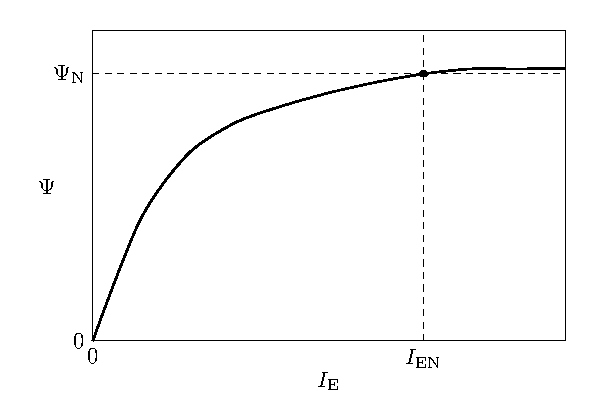
\includegraphics[width=0.65\textwidth]{./bilder/aufgabe5_skript.pdf}
	\caption{Prinzipieller Zusammenhang $ \psi(I_{E}) $ ohne Hysterese, Quelle: \textquotedblleft Elektische Antriebe: Vorlesung zum Sommersemester 2018\textquotedblright, \textit{Prof.–Dr.–Ing. Gernot Schullerus}}
	\label{fig:5:skript}
\end{figure}


\section{}
Wenn man den Erregerstrom $ I_{E} $ herabsetzt, wandert der Betriebspunkt des Motors in den Feldschwächebereich. Die Last kann im Feldschwächebereich jedoch nicht mehr so hoch gewählt werden, trotz dessen dass die Drehzahl des Motors ansteigt. Wird ein kritischer Punkt von $ I_{E} $ unterschritten, so wird die Drehzahl des Motors ins unendliche steigen. Dies führt unweigerlich zur mechanischen Selbstzerstörung des Motors.


\section{}
In diesem Aufgabenteil soll die Magnetisierungskennlinie durch eine Exceltabelle mit unseren Messwerten dargestellt werden. Wie in der Aufgabe 4 b) wollen wir hier auch kein Ankerstrom haben. Deshalb haben wir unseren GM mit unserer Lastmaschine betrieben. Dabei haben wir die Drehzahl N konstant auf 1000 Umdrehungen pro Minunte und den Ankerstrom mit einem Intervervall von 0,05A von 0 auf 0,5 A gesetzt. Die Ankerspannung haben wir nach jedem Intervall mit einem Multimeter ausgelesen und diese alle in der Tabelle \ref{tab:5c:cepsi} dargestellt. Anschließend haben wir die Werte in einem Diagramm Abbildung \ref{fig:5c:kennlinie}) dargestellt.  
\begin{table}[h]
	\centering
	\begin{tabular}{p{1.5cm} p{1.5cm} p{1.5cm} p{1.5cm} | p{1.5cm}}
		&&&&\\[-1em]
		$ U_{A}/V $ & $ I_{E} $ & $ N/min^{-1} $ & $ N/s^{-1} $ &  $ c_{E}\Psi/Vs $\\
		\hline &&&&\\[-1em]
		50.5 & 0.47 & 1000 & 16.7 & 3.030\\
		50.1 & 0.45 & 1000 & 16.7 & 3.006\\
		48.8 & 0.40 & 1000 & 16.7 & 2.928\\
		47.4 & 0.35 & 1000 & 16.7 & 2.884\\
		45.5 & 0.30 & 1000 & 16.7 & 2.730\\
		42.9 & 0.25 & 1000 & 16.7 & 2.574\\
		39.1 & 0.20 & 1000 & 16.7 & 2.346\\
		33.0 & 0.15 & 1000 & 16.7 & 1.980\\
		24.2 & 0.10 & 1000 & 16.7 & 1.452\\
		13.2 & 0.05 & 1000 & 16.7 & 0.792\\
		2.0 & 0.00 & 1000 & 16.7 & 0.120		
	\end{tabular}
	\caption{Messwerte für die Magnetisierungskennlinie }
	\label{tab:5c:cepsi}
\end{table}


\begin{figure}[h]
	\centering
	% This file was created by matlab2tikz.
%
%The latest updates can be retrieved from
%  http://www.mathworks.com/matlabcentral/fileexchange/22022-matlab2tikz-matlab2tikz
%where you can also make suggestions and rate matlab2tikz.
%
\definecolor{mycolor1}{rgb}{0.00000,0.44700,0.74100}%
%
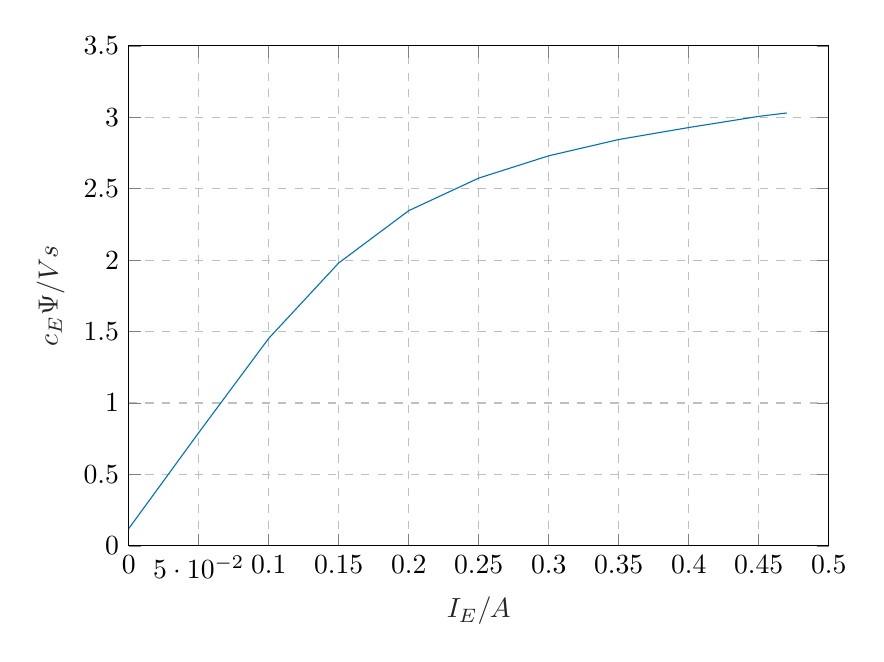
\begin{tikzpicture}

\begin{axis}[%
width=3.5in,
height=2.5in,
at={(0.758in,0.481in)},
scale only axis,
xmin=0,
xmax=0.5,
xtick={   0, 0.05,  0.1, 0.15,  0.2, 0.25,  0.3, 0.35,  0.4, 0.45,  0.5},
xlabel style={font=\color{white!15!black}},
xlabel={$ I_{E}/A $},
ymin=0,
ymax=3.5,
ytick={  0, 0.5,   1, 1.5,   2, 2.5,   3, 3.5},
ylabel style={font=\color{white!15!black}},
ylabel={$ c_{E}\Psi/Vs $},
axis background/.style={fill=white},
xmajorgrids,
ymajorgrids,
major grid style={dashed}
]
\addplot [color=mycolor1]
  table[row sep=crcr]{%
0	0.12\\
0.05	0.792\\
0.1	1.452\\
0.15	1.98\\
0.2	2.346\\
0.25	2.574\\
0.3	2.73\\
0.35	2.844\\
0.4	2.928\\
0.45	3.006\\
0.47	3.03\\
};

\end{axis}
\end{tikzpicture}%
	\caption{Kurve der Magnetisierungskennlinie}
	\label{fig:5c:kennlinie}
\end{figure}


\section{}
In den letzten Aufgabenteil soll der Nennpunkt in die Magnetisierungskennlinie eingezeichnet werden und es soll begründet werden, warum der Nennfluss in diesem Bereich festgelegt liegt. Die Arbeitspunkte $ I_{E1} = I_{EN} $ und $ I_{E2} = \frac{1}{2} I_{EN} $ sind auch zu vergleichen.
Der Nennpunkt liegt in unsere Magnetisierungskennlinie am Arbeitspunkt $ I_{E1} = I_{EN} $ (Abbildung \ref{fig:5d:kennlineNenn}). Diese haben wir so bestimmt, indem wir den Erregerstrom so weit erhöht haben, bis sich die Ankerspannung nicht mehr ändert. Dies ist bei $ I_{EN} = 0.47A $ der Fall.
\begin{figure}[h]
	\centering
	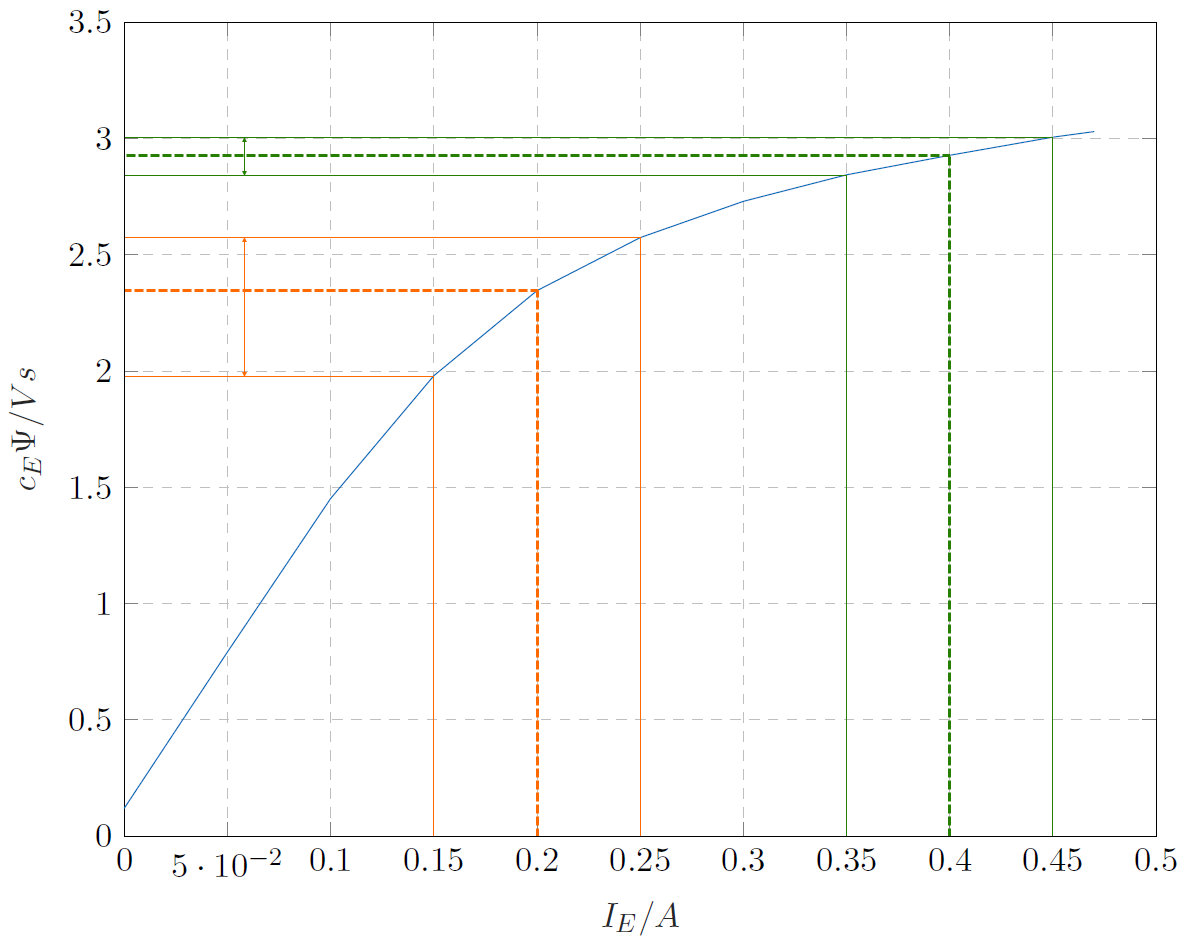
\includegraphics[width=0.7\textwidth]{./bilder/aufgabe4.png}
	\caption{Kurve der Magnetisierungskennlinie mit Nennpunkt}
	\label{fig:5d:kennlineNenn}
\end{figure}

Damit wir den erforderlichen Ankerstrom in den jeweiligen Arbeitspunkte bestimmen können, nehmen wir die Gleichung (\ref{eq:5d:mn}) und formen es nach $ I_{A} $ (\ref{eq:5d:ia}) um. Das Nennmoment $ M_{N} $ haben wir aus den Daten auf dem Leistungsschild berechnet. Näheres dazu wird in der Aufgabenstellung 6 erläutert.
\begin{equation}
	M_{N} = c_{M}\psi I_{A}
	\label{eq:5d:mn}
\end{equation} und stellen nach $ I_{A} $ um, somit ergibt sich die Formel:
\begin{equation}
	I_{A} = \frac{2\pi M_{N}}{c_{E}\psi}
	\label{eq:5d:ia}
\end{equation}
Die Werte in unsere Gleichung eingesetzt ergibt:
\begin{center}
	$ I_{A}(I_{E1}) = \frac{2\pi *1.75Nm}{2.5Vs} = 4.40A $ \\
	$ I_{A}(I_{E2}) = \frac{2\pi *1.75Nm}{3.03Vs} = 3.63A $
\end{center}

In der Abbildung \ref{fig:5d:kennlineNenn} kann man im Arbeitspunkt $ I_{E1} $ erkennen, dass bei Änderungen von $ I_{E} $ von +-50mA, $ \Delta\psi $ deutlich kleiner ist, als im Arbeitspunkt $ I_{E2} $. Somit ist der AP1 günstiger, da es zum einen geringeren Ankerstrom erzeugt und sich somit die Maschine langsamer erwärmt - man muss die GM weniger kühlen. Auch kann man einen kleineren Querschnittsfläche für die Drähte, wegen des kleineren Ankerstroms benutzen. Die geringe Änderung von $ I_{E1} $ heißt auch, dass sie einen geringeren Einfluss auf den Fluss hat und es zu einer stabileren Drehzahl der Gleichstrommaschine führt.